\chapter[\CP-Verletzung im B-Meson-System]{\CP-Verletzung im B-Meson-System} \label{kap:cp-verletzung}
\section{Das Standardmodell der Teilchenphysik}
Im Standardmodell der Teilchenphysik gibt es 17 elementare Bausteine der Materie (siehe Abb. \ref{fig:standardmodell}): 12 Fermionen, davon 6 Quarks (u, d, c, s, t, b), die sich im engeren Sinne zur Materie hadronisieren oder Mesonen bilden, und 6 Leptonen (e, $\mu$, $\tau$ sowie die jeweiligen Neutrinos $\nu_{\text{e}}$, $\nu_{\mu}$, $\nu_{\tau}$). Von diesen 12 Fermionen existieren jeweils noch Antiteilchen (gleiche Masse, aber entgegengesetzte Quantenzahlen). Das Standardmodell enthält weiterhin 4 Eichbosonen (Photon, Gluon, Z- und W$^{\pm}$-Boson), die die 3 der 4 elementaren Kräfte übertragen: die elektromagnetische, starke und schwache Wechselwirkung. Die Gravitation als vierte elementare Kraft wird nicht durch das Standardmodell beschrieben. Ergänzt wird das Standardmodell durch das Higgs-Boson, welches als Teil des Higgs-Mechanismus den Elementarteilchen seine Masse verleiht und Gegenstand aktueller Forschung ist. Mit hoher Wahrscheinlichkeit gelang jüngst der Nachweis des Higgs am CERN \cite{higgs}.
\begin{figure}[hptb]
\centering
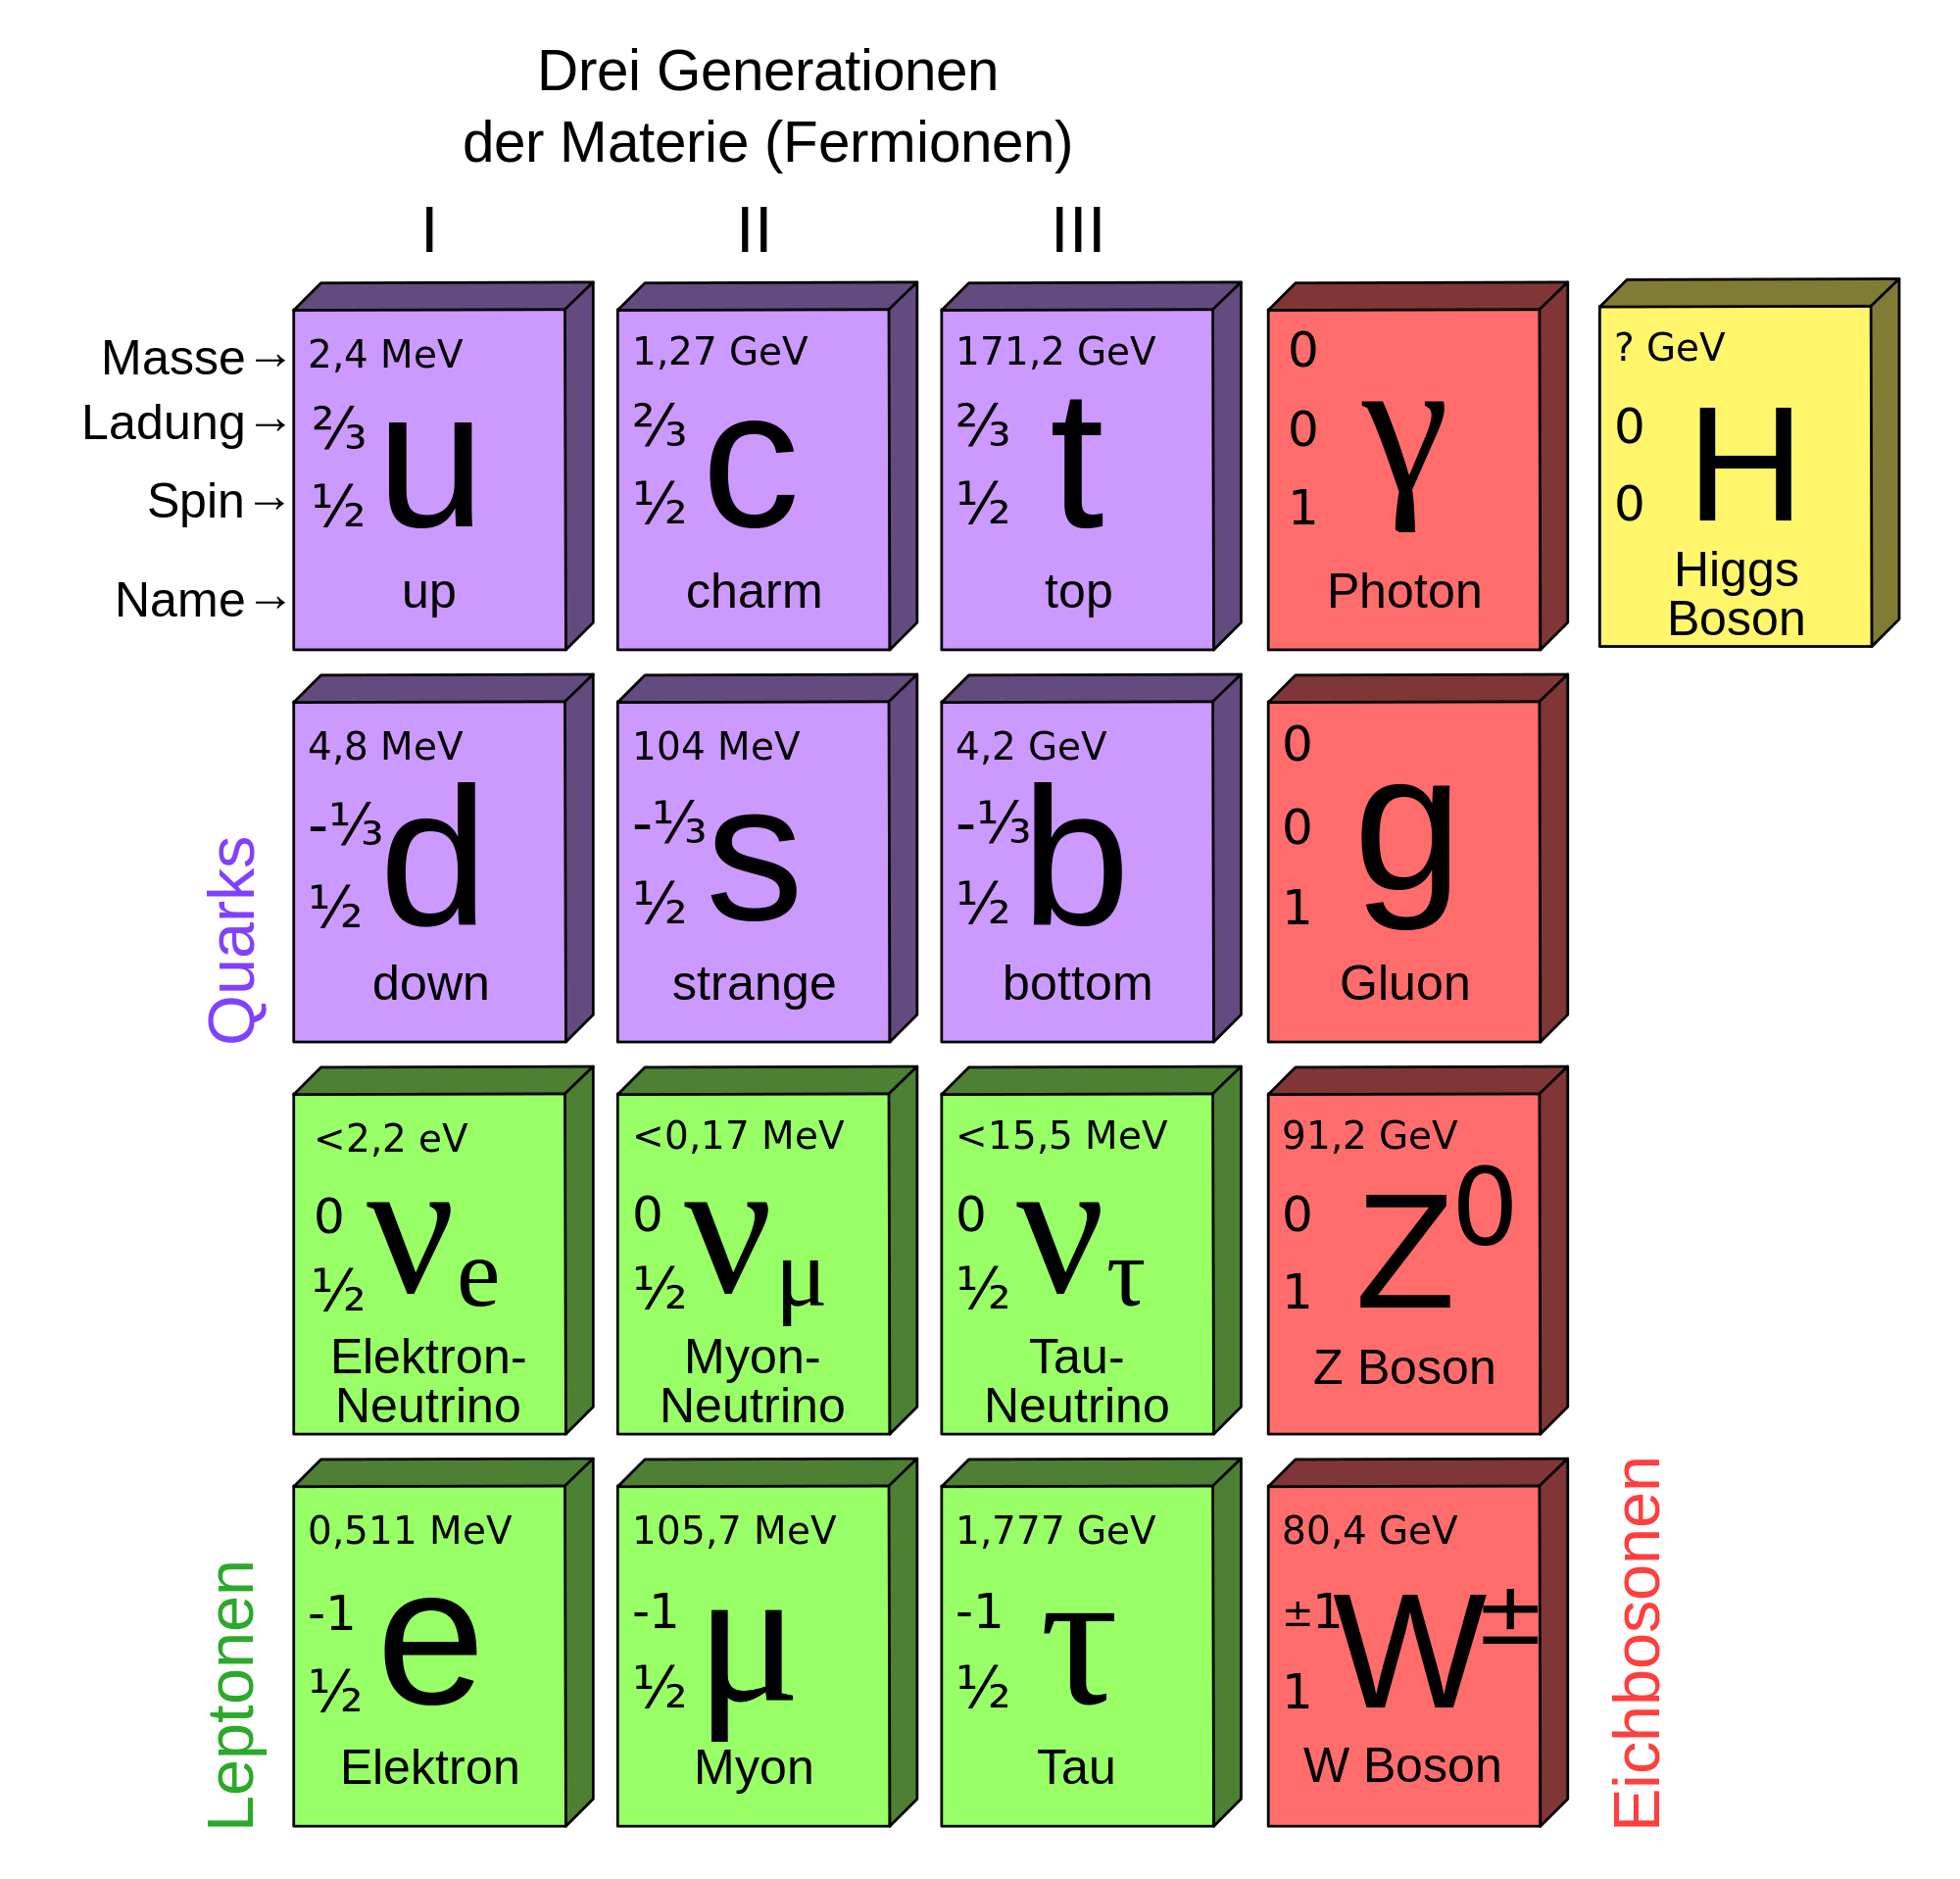
\includegraphics[width=0.5\textwidth]{standardmodell}
\caption{Die Bausteine / Teilchen des Standardmodells. Abbildung entnommen aus \cite{wiki_standard}.}
\label{fig:standardmodell}
\end{figure}

\section{B-Mesonen und ihre Mischung}
Mesonen sind Paare aus Quarks und Antiquarks beliebigen Flavours. B-Mesonen insbesondere bestehen aus einem Anti-b-Quark ($\mathrm{\overline{b}}$) mit einem u-, d-, c- oder s-Quark, Anti-B-Mesonen entsprechend aus der Kombination der jeweiligen Antiteilchen. Die in dieser Arbeit betrachteten \Bd-Mesonen haben demnach die Quarkzusammensetzung $\Ket{\text{\Bd}} = \Ket{\overline{b}d}$ und sind elektrisch neutral. Solch neutrale Mesonen besitzen die Eigenschaft, dass sie sich in ihre Antiteilchen wandeln können und umgekehrt. Es findet folglich eine Oszillation zwischen \Bd\ und \Bdbar\ statt, die man auch Mischung nennt. Abbildung \ref{fig:bmixing} zeigt zwei mögliche Feynmangraphen für diesen Prozess. Innerhalb der Schleifen kann nach Heisenberg die Energieerhaltung kurzzeitig verletzt werden, sodass auch kurzerhand bspw. die deutlich schwereren top-Quarks enstehen können. Ebenso ist es vorstellbar, dass bislang unentdeckte, noch schwerere Teilchen beitragen können. Präzise Messungen der \Bd-Mischung erlauben Aussagen bspw. über die top-Masse und grenzen damit das Standardmodell ein. Gleichzeitig erhofft man sich, durch noch präzisere Messungen Hinweise auf \glqq neue Physik\grqq\ zu finden, die sich dann, wie bereits erwähnt, in kleinsten Korrekturen innerhalb der Schleife bemerkbar machen würden.

\begin{figure}[hptb]
\centering
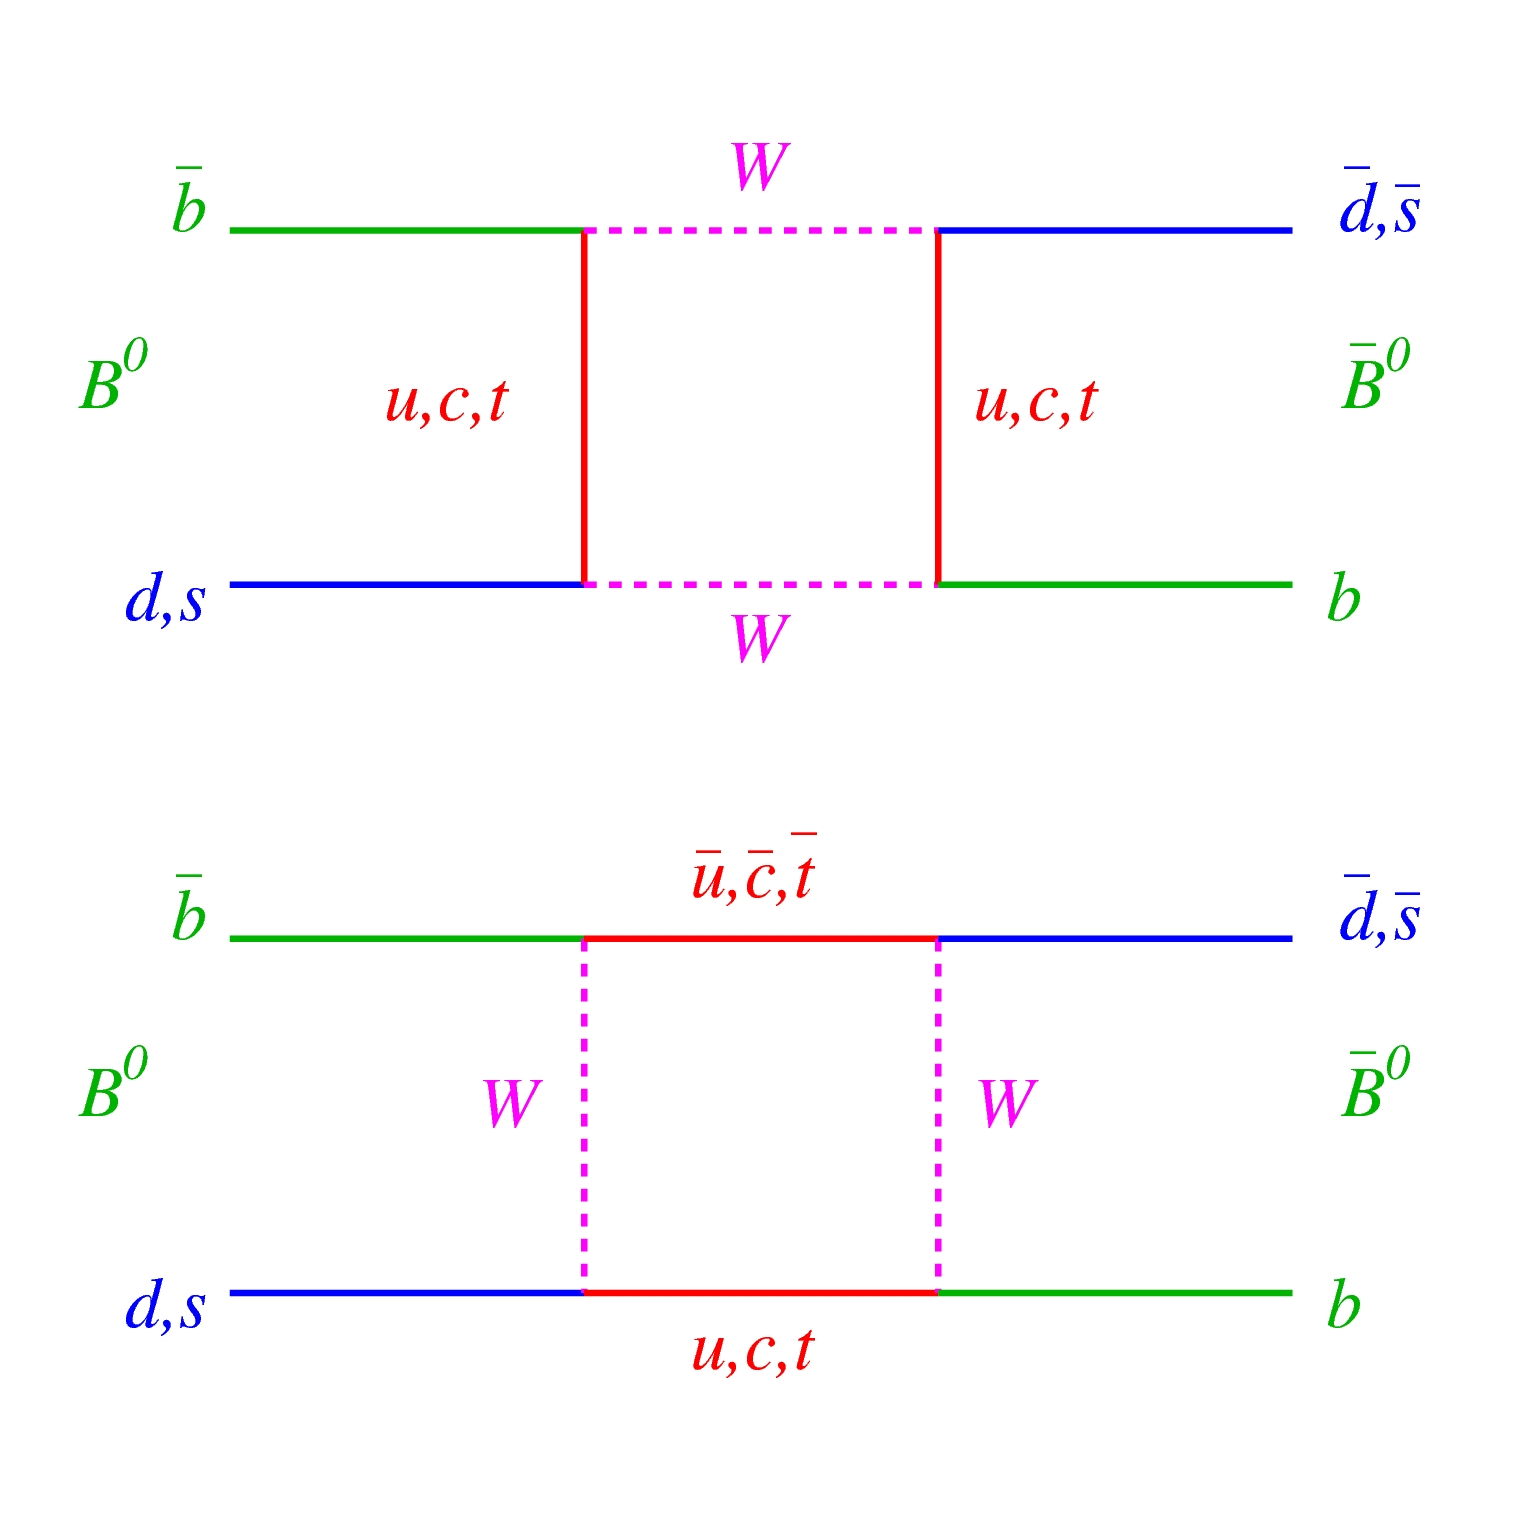
\includegraphics[width=\textwidth]{bmixing}
\caption{Feynmangraphen zur Mischung von \Bd- und \Bdbar-Mesonen. Dabei repräsentiert $q$ ein $d$- bzw. $s$-Quark. Die Abbildung wurde \cite{roadmap} entnommen.}
\label{fig:bmixing}
\end{figure}


\section[Der Zerfallskanal \Decaychannel]{Der Zerfallskanal \boldmath\Decaychannel\unboldmath}
In dieser Arbeit wird der Zerfallskanal \Decaychannel\ betrachtet. Abbildung \ref{fig:decay} zeigt entsprechende Feynmangraphen. Jener Kanal ist auch als \glqq goldener\grqq\ Zerfallskanal für die Messung der \CP-Verletzung bekannt. Hintergrund ist, dass der vom Baumdiagramm (Abb. \ref{fig:decay}, links) beschriebene Prozess dominiert und damit \CP-Verletzung im Zerfall vernachlässigbar ist. Des Weiteren hat dieser Zerfall ein hohes Verzweigungsverhältnis, womit mehr Statistik als in anderen Kanälen zur Verfügung steht. Der Endzustand $\Ket{\JPsi\Kshort}$ ist näherungsweise ein \CP-Eigenzustand ($\text{\CP}\Ket{\JPsi\Kshort} = - \Ket{\JPsi\Kshort}$). Damit können sowohl \Bd- als auch \Bdbar-Mesonen in den Endzustand zerfallen. Da \Bd\ und \Bdbar\ auch noch mischen, kommt es zu \CP-verletzenden Interferenzen der Zerfallsamplituden für den direkten Zerfall und den Zerfall nach vorheriger Mischung. Die Teilchen $\JPsi$ und $\Kshort$ haben die Flavoureigenzustände $\Ket{\JPsi} = \Ket{c\overline{c}}$ sowie $\Ket{\Kshort} = \tfrac{1}{\sqrt{2}}\left(\Ket{d\overline{s}}-\Ket{s\overline{d}}\right)$\footnote{Beim Flavoureigenzustand wurde eine kleine Korrektur auf Grund von \CP-Verletzung im Kaon-System vernachlässigt. Zur vollständigen Korrektheit müsste weiterhin in Abbildung \ref{fig:decay} statt dem $\Kshort$ lediglich ein $K^0$ stehen. Das entsprechende \Bdbar\ hätte dann ein $\overline{K^0}$ als Endprodukt. Die Argumentation, dass sowohl \Bd\ als auch \Bdbar\ in den selben Endzustand zerfallen ist dennoch richtig, da auch die $K^0-/\overline{K^0}$-Mischung existiert.}. Diese Teilchen sind ebenfalls nicht stabil und zerfallen unter anderem weiter gemäß $\JPsi \rightarrow \mu^+\mu^-$ und $\Kshort \rightarrow \pi^+\pi^-$, was zur Rekonstruktion der \Bd-Mesonen im Detektor genutzt wird.

\begin{figure}[hptb]
\centering
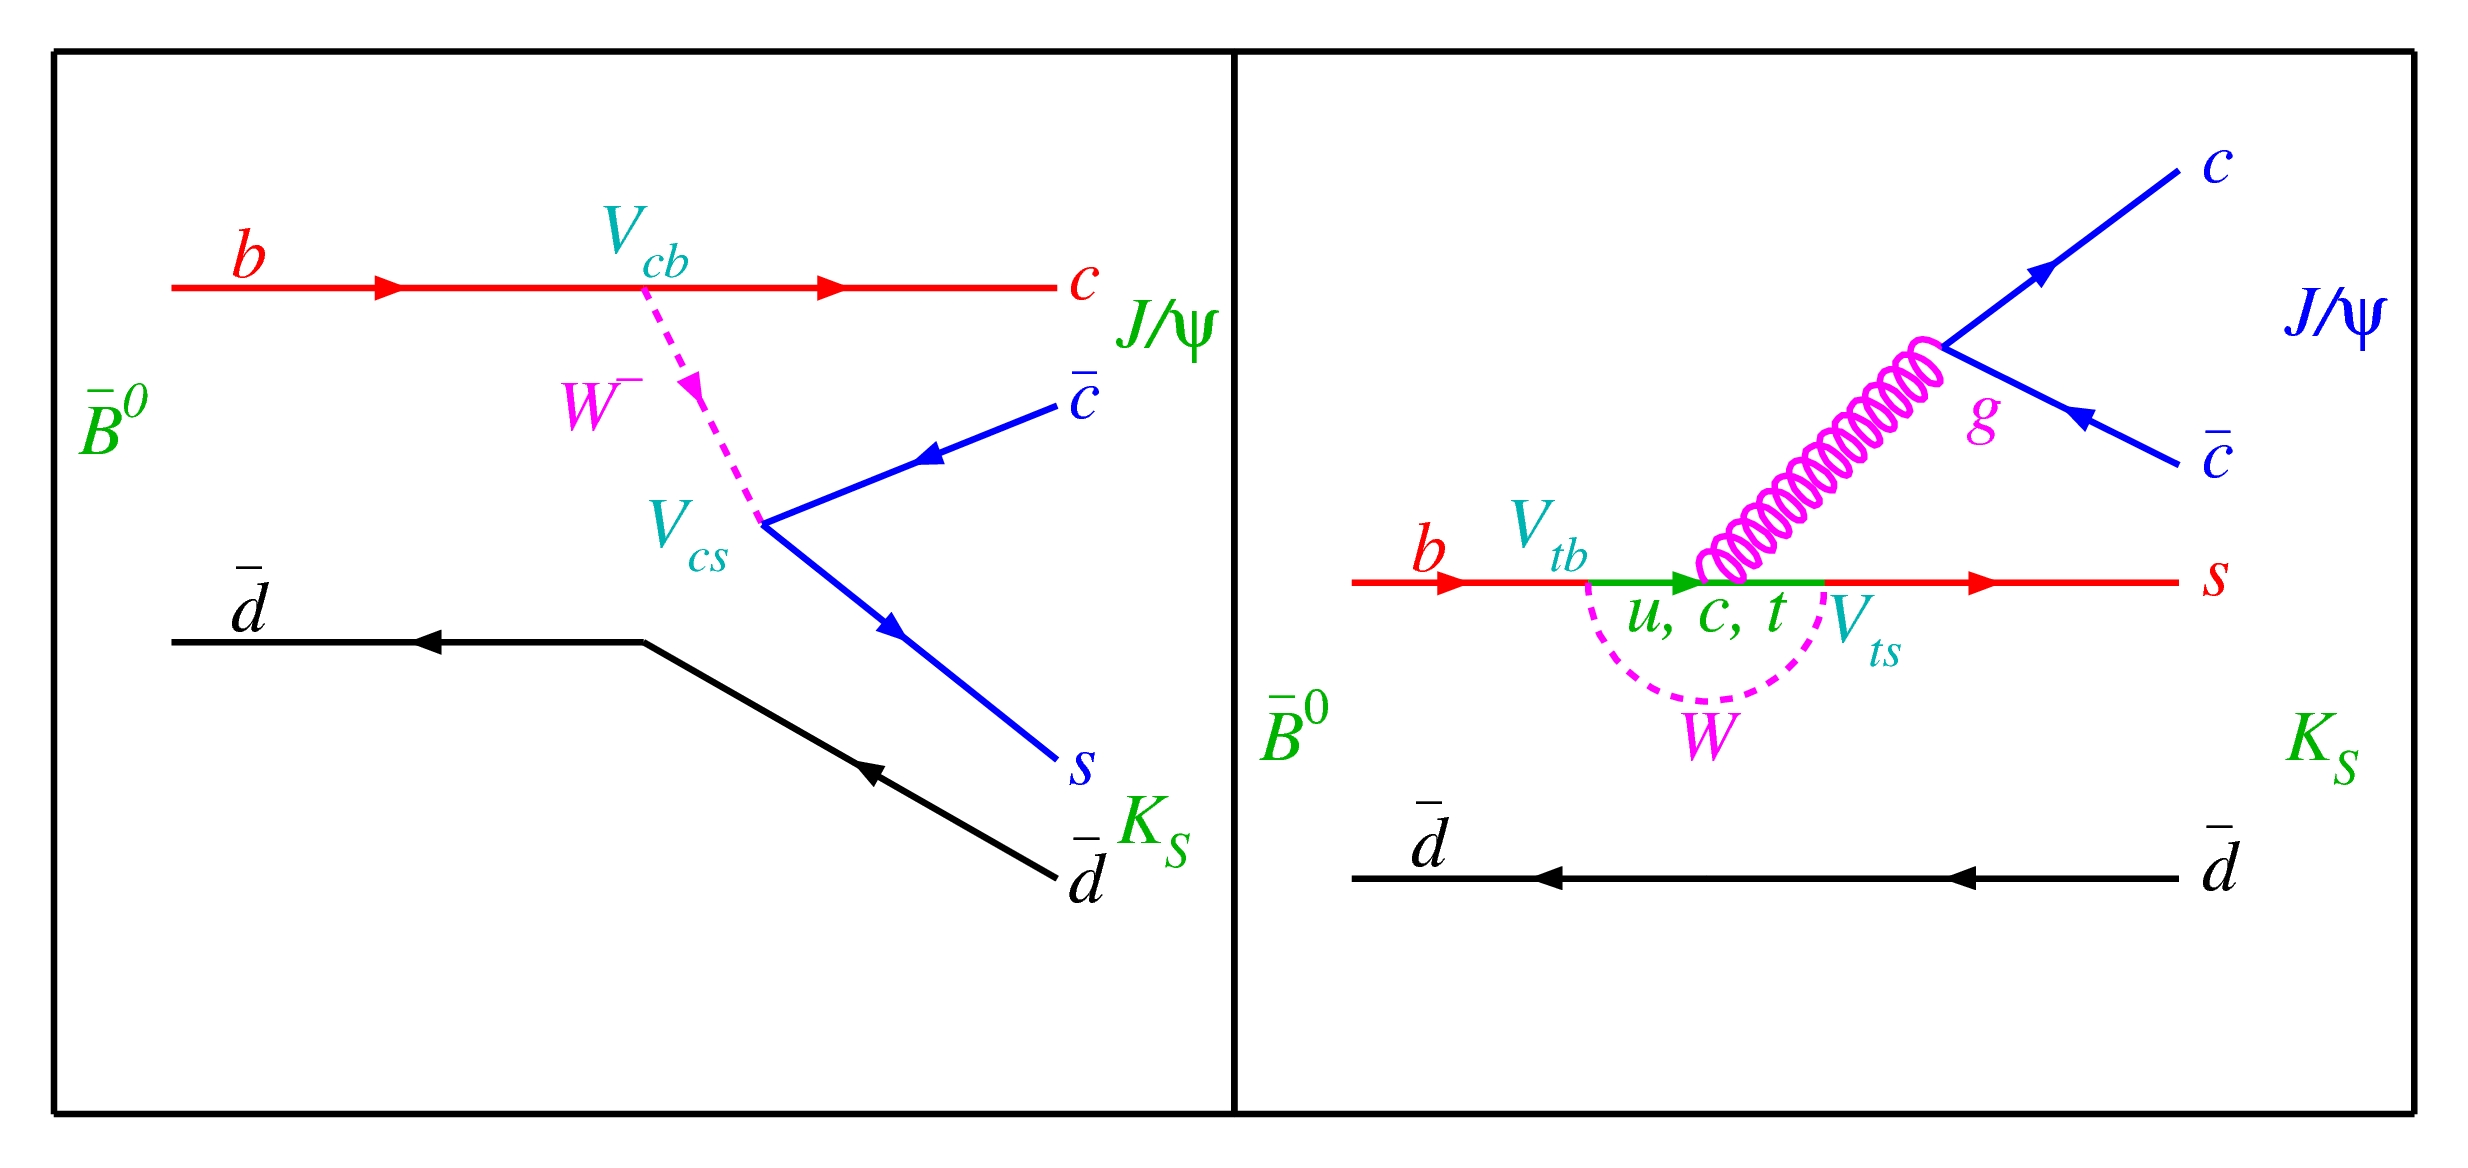
\includegraphics[width=\textwidth]{bd2jpsikshort}
\caption{Feynmangraph zum Zerfall \Decaychannel. Links: Baumdiagramm, rechts: Pinguindiagramm (stark unterdrückter Prozess). Die Abbildung wurde \cite{lhcb-paper} entnommen.}
\label{fig:decay}
\end{figure}

\section{Diskrete Symmetrietransformationen}
Symmetrien sind in der Physik von zentraler Bedeutung. Gemäß dem Noether-Theorem existiert in der klassischen Physik zu jeder kontinuierlichen Symmetrie eine Erhaltungsgröße. In quantenmechanischen Systemen lassen sich drei diskrete Symmetrietransformationen betrachten:
\begin{enumerate}
\boldmath
\item \textbf{Parität $\mathcal{P}$:} \\
      Bei der Paritätsoperation wird das Vorzeichen der kartesischen Ortskoordinaten umgekehrt. Dies entspricht einer Punktspigelung.
\item \textbf{Ladungskonjugation $\mathcal{C}$:} \\
      Jedes Teilchen wird durch sein Antiteilchen ersetzt.
\item \textbf{Zeitumkehr $\mathcal{T}$:} \\
      Das Vorzeichen auf der Zeitachse wird umgekehrt. Da in der vorliegenden Arbeit allerdings nur die \CP-Verletzung gemessen werden soll, wird die Zeitumkehr im Folgenden vernachlässigt.
\unboldmath
\end{enumerate}
Entgegen der klassischen Intuition konnte Wu 1956 nachweisen \cite{wu-experiment}, dass die Parität im $\beta$-Zerfall und damit in der schwachen Wechselwirkung nicht erhalten ist. Weitere Experimente zeigen, dass die schwache Wechselwirkung die Parität maximal verletzt: Neutrinos, die nur schwach wechselwirken können, sind stets \glqq linkshändig\grqq\ (Spin und Impuls antiparallel), Antineutrinos dagegen immer \glqq rechtshändig\grqq\ (Spin und Impuls parallel). Da der Spin im Gegensatz zum Impuls invariant unter $\mathcal{P}$-Transformation ist, würde diese Operation aus einem linkshändigen Neutrino ein rechtshändiges machen, was in der Natur nicht realisiert ist.

Damit ist offensichtlich, dass die schwache Wechselwirkung auch die Ladungskonjugation verletzt: Wendet man die $\mathcal{C}$-Transformation auf ein linkshändiges Neutrino an, so erhält man ein linkshändiges Antineutrino. Dieses existiert aber wie bereits erwähnt nicht. Analog gilt die Überlegung auch für Antineutrinos.

\subsubsection{Scheinbare \boldmath$\mathcal{CP}$\unboldmath-Invarianz}
Wendet man nun aber die Transformationen $\mathcal{P}$ und $\mathcal{C}$ direkt hintereinander an, so ergibt sich kein Widerspruch zur Natur (siehe Abb. \ref{fig:cp_invarianz}). Aus einen linkshändigen Neutrino wird ein rechtshändiges Antineutrino. Es erscheint, als sei \CP\ die wahre Symmetrietransformation. Im Jahre 1964 wurde dann allerdings im Zerfall neutraler K-Mesonen erstmals $\mathcal{CP}$-Verletzung nachgewiesen \cite{kleinknecht}.
\begin{figure}[hptb]
\centering
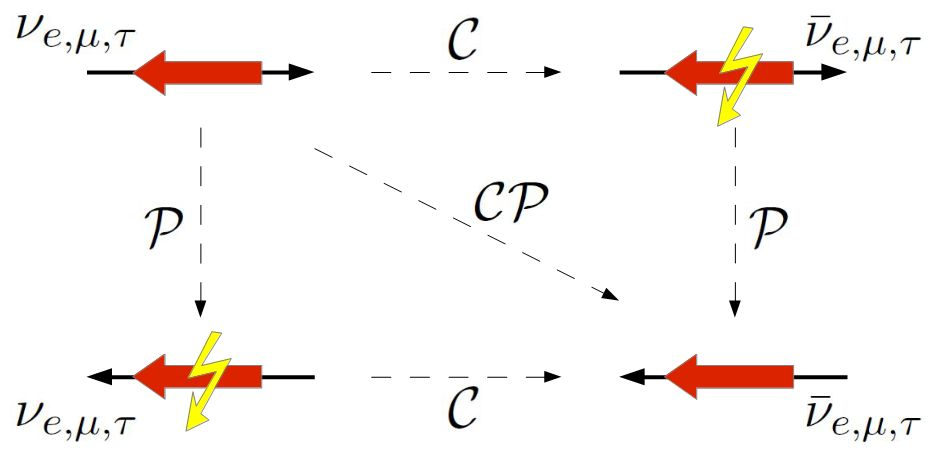
\includegraphics[width = 0.8\textwidth]{cp_invarianz}
\caption{Scheinbare $\mathcal{CP}$-Invarianz: Während eine reine $\mathcal{P}$- oder $\mathcal{C}$-Transformation zu in der Natur nicht realisierten Zuständen führt, scheint es bei der kombinierten $\mathcal{CP}$-Transformation keinen Widerspruch zu geben (dünne Pfeile: Impulsausrichtung, dicke Pfeile: Spinausrichtung).}
\label{fig:cp_invarianz}
\end{figure}
Diese Arbeit beschäftigt sich mit der \CP-Verletzung im B-Mesonen-System. Eine genaue Kenntnis der \CP-Verletzung ermöglicht Präzisionstests des Standardmodells. Weiterhin ist insbesondere das B-Meson-System sensitiv für \glqq neue Physik\grqq, da durch Schleifen innerhalb der Prozesse (siehe Abb. \ref{fig:bmixing} und \ref{fig:decay}) Beiträge von Theorien jenseits des Standardmodells möglich sind und evtl. zu Abweichungen führen. Dabei unterscheidet man prinzipiell drei Arten von \CP-Verletzung:
\begin{enumerate}
\item \textbf{\boldmath\CP-Verletzung in der Mischung (auch indirekte \CP-Verletzung):\unboldmath} \\
      Sie tritt immer dann auf, wenn die Masseneigenzustände eines neutralen Meson-Systems nicht den \CP-Eigenzuständen entsprechen. In der Folge ist die Rate der Oszillationen beispielsweise eines \Bd\ in ein \Bdbar\ unterschiedlich von der eines \Bdbar\ in ein \Bd.
\item \textbf{Direkte \boldmath\CP-Verletzung:\unboldmath} \\
      Sie tritt dann auf, wenn sich die Zerfallsamplitude eines B-Mesons in eines Endzutand $f$ von der (\CP-konjugierten) Zerfallsamplitude des Anti-B-Mesons in den Zustand $\overline{f}$ unterscheidet. Demnach sind dann die partiellen Breiten der direkten Zerfälle unterschiedlich: $\Gamma (\text{B} \rightarrow f) \neq \Gamma (\overline{\text{B}} \rightarrow \overline{f})$.
\item \textbf{\boldmath\CP-Verletzung in der Interferenz zwischen Mischung und Zerfall:\unboldmath} \\
      Sie kommt dadurch zum Ausdruck, dass der zeitabhängige Zerfall eines anfänglich reinen Flavourzustandes für ein Teilchen und ein Antiteilchen unterschiedlich ist. Diese Art der \CP-Verletzung kann bei neutralen Mesonen auftreten, wenn der Endzustand ein \CP-Eigenzustand ist. Hintergrund ist, dass es zu \CP-verletzenden Interferenzen der Zerfallsamplituden für direkten Zerfall (z.B. $\text{\Bd} \rightarrow \JPsi\Kshort$) und Zerfall nach Mischung ($\text{\Bd} \rightarrow \text{\Bdbar} \rightarrow \JPsi\Kshort$) kommt.
\end{enumerate}
Die nun folgenden Herleitungen und Erklärungen der drei Arten der \CP-Ver\-let\-zung basieren auf den Ausführungen aus \cite{kleinknecht}.

\section[\CP-Verletzung in der Mischung]{\boldmath\CP-Verletzung\ \unboldmath in der Mischung}
Die Zeitentwicklung der Flavoureigenzustände zum Zeitpunkt $t=0$, $\Ket{\text{\Bd}\vphantom{\text{\Bdbar}}} = \Ket{\overline{b}d\vphantom{\text{\Bdbar}}}$ und $\Ket{\text{\Bdbar}} = \Ket{b\overline{d}\vphantom{\text{\Bdbar}}}$, die sich unter \CP-Transformation gemäß
\begin{align}
\text{\CP}\Ket{\text{\Bd}\vphantom{\text{\Bdbar}}} = \e^{\im\phi}\Ket{\text{\Bdbar}} \qquad \text{\CP}\Ket{\text{\Bdbar}} = \e^{-\im\phi}\Ket{\text{\Bd}\vphantom{\text{\Bdbar}}}
\end{align} 
mit einer willkürlichen Phase $\phi$ verhalten, lässt sich phänomenologisch durch die Schrödinger-Gleichung
\begin{align}
\im \diff{}{t}\begin{pmatrix} \Ket{\text{\Bd}\vphantom{\text{\Bdbar}}} \\ \Ket{\text{\Bdbar}} \end{pmatrix} = \left(M - \frac{\im}{2} \Gamma\right) \begin{pmatrix} \Ket{\text{\Bd}\vphantom{\text{\Bdbar}}} \\ \Ket{\text{\Bdbar}} \end{pmatrix}
\end{align}
beschreiben. Der Hamiltonoperator $\mathcal{H}:=\left(M - \frac{\im}{2} \Gamma\right)$ setzt sich zusammen aus dem hermiteschen Massenoperator $M$ und dem ebenfalls hermiteschen Zerfallsoperator $\Gamma$. $\mathcal{H}$ selbt ist nicht hermitesch wegen des möglichen Zerfalls des Teilchens. Aus der $\mathcal{CPT}$-Erhaltung folgt $M_{11}=M_{22}=:M$ bzw. $\Gamma_{11}=\Gamma_{22}=:\Gamma$. Die nichtverschwindenden Elemente abseits der Diagonalen $M_{12}=M_{21}^*$, $\Gamma_{12}=\Gamma_{21}^*$ parametrisieren die \Bd-\Bdbar-Mischung. Offensichtlich entsprechen die Flavoureigenzustände nicht den Eigenzuständen von $\mathcal{H}$. Diagonalisieren von $\mathcal{H}$ liefert die Eigenzustände
\begin{align}
\Ket{B_{\text{H}}\vphantom{\text{\Bdbar}}} &= p \Ket{\text{\Bd}\vphantom{\text{\Bdbar}}} - q \Ket{\text{\Bdbar}} \label{eq:b_heavy}\\ 
\Ket{B_{\text{L}}\vphantom{\text{\Bdbar}}} &= p \Ket{\text{\Bd}\vphantom{\text{\Bdbar}}} + q \Ket{\text{\Bdbar}}, \qquad \text{mit} \quad |p|^2 + |q|^2 = 1, \label{eq:b_light}
\end{align}
mit definierten Massen $m_{\text{H/L}}$ und Zerfallsbreiten $\Gamma_{\text{H/L}}$ sowie den Eigenwerten  $m_{\text{H/L}}-\frac{\im}{2}\Gamma_{\text{H/L}}$. Die Indizierung orientiert sich an den Masseneigenwerten, dabei steht $\text{H}$ für den schweren (engl. heavy) und $\text{L}$ für den leichten (engl. light) Zustand. Aus den Eigenwerten von $\mathcal{H}$ folgt die zeitliche Entwicklung der Zustände:
\begin{align}
\nonumber \Ket{B_{\text{H/L}}(t)\vphantom{\text{\Bdbar}}} &= \e^{-\im m_{\text{H/L}}t-\frac{1}{2}\Gamma_{\text{H/L}}t}\Ket{B_{\text{H/L}}(0)\vphantom{\text{\Bdbar}}} \\
                           &= \e^{-\gamma_{\text{H/L}}t}\left(p\Ket{\text{\Bd}\vphantom{\text{\Bdbar}}} \mp q\Ket{\text{\Bdbar}}\right), \qquad
 \text{mit} \quad \gamma_{\text{H/L}} = \im m_{\text{H/L}}+\frac{\Gamma_{\text{H/L}}}{2}
\end{align}
Umgeschrieben auf die Flavoureigenbasis erhält man:
\begin{align}
\nonumber \Ket{\text{\Bd}(t)\vphantom{\text{\Bdbar}}} &= \frac{1}{2p}\left(\Ket{B_{\text{H}}\vphantom{\text{\Bdbar}}} + \Ket{B_{\text{L}}\vphantom{\text{\Bdbar}}}\right) \\
                       &= \frac{1}{2}\left[ (\e^{-\gamma_{\text{H}} t}+\e^{-\gamma_{\text{L}} t})\Ket{\text{\Bd}\vphantom{\text{\Bdbar}}} - \frac{q}{p}(\e^{-\gamma_{\text{H}} t}-\e^{-\gamma_{\text{L}} t})\Ket{\text{\Bdbar}}\right] \label{eg:b(t)}
\end{align}
Die Wahrscheinlichkeit für den Übergang eines $\Ket{\text{\Bd}\vphantom{\text{\Bdbar}}}$ (zum Zeitpunkt $t=0$) in ein $\Ket{\text{\Bdbar}}$ beträgt:
\begin{align}
\nonumber P(\text{\Bd}\rightarrow\text{\Bdbar})(t) &= \left|\Braket{\text{\Bdbar}|\text{\Bd}(t)}\right|^2 \\
                                        &= \frac{1}{4} \left|\frac{q}{p}\right|^2 \left[\e^{-\Gamma_{\text{H}} t} + \e^{-\Gamma_{\text{L}} t} - 2\e^{-\frac{1}{2}(\Gamma_{\text{H}} + \Gamma_{\text{L}}) t}\cos(\Delta m_d t)\right]
\end{align}
Hierbei wird die Oszillationsdifferenz $\Delta m_d := m_{\text{H}} - m_{\text{L}}$ definiert, die aus der Massendifferenz der beiden Masseneigenzustände resultiert. Analog gilt für die Übergangswahrscheinlichkeit eines $\Ket{\text{\Bdbar}}$ in ein $\Ket{\text{\Bd}\vphantom{\text{\Bdbar}}}$:
\begin{align}
P(\text{\Bdbar}\rightarrow \text{\Bd})(t) = \frac{1}{4} \left|\frac{p}{q}\right|^2 \left[\e^{-\Gamma_{\text{H}} t} + \e^{-\Gamma_{\text{L}} t} - 2\e^{-\frac{1}{2}(\Gamma_{\text{H}} + \Gamma_{\text{L}}) t}\cos(\Delta m_d t)\right] 
\end{align}
Folglich kommt es in der Mischung zur \CP-Verletzung, wenn die Oszillation ungleichmäßig verläuft, anders ausgedrückt:
\begin{align}
\text{\CP-Verletzung in der Mischung} \qquad \Longleftrightarrow \qquad \left|\frac{p}{q}\right| \neq 1 
\end{align}

\section[Direkte \CP-Verletzung]{Direkte \boldmath\CP-Verletzung\unboldmath}
Die Zerfallsamplituden der neutralen $\text{\Bd}$-Mesonen in einen Endzustand $\Ket{f}$ bzw. seinen \CP-konjugierten Zustand $\Ket{\overline{f}}$ sind definiert als
\begin{alignat}{2}
\nonumber A_f &= \Braket{f|\mathcal{H}|\text{\Bd}\vphantom{\text{\Bdbar}}}, && \qquad A_{\overline{f}} = \Braket{\overline{f}|\mathcal{H}|\text{\Bd}\vphantom{\text{\Bdbar}}}, \\
          \overline{A_f} &= \Braket{f|\mathcal{H}|\text{\Bdbar}}, && \qquad  \overline{A_{\overline{f}}} = \Braket{\overline{f}|\mathcal{H}|\text{\Bdbar}}. \label{eq:decay_amplitudes}
\end{alignat}
Ist \CP\ erhalten, dann sollten die Zerfallsraten, ergo auch die Zerfallsamplituden eines $\text{\Bd}$ nach $f$ sowie eines $\text{\Bdbar}$ nach $\overline{f}$ gleich sein. Dies bedeutet:
\begin{align}
\text{Direkte \CP-Verletzung} \qquad \Longleftrightarrow \qquad \frac{|A_f|}{|\overline{A_{\overline{f}}}|} \neq 1 \quad \text{bzw.} \quad \frac{|\overline{A_f}|}{|A_{\overline{f}}|} \neq 1
\end{align}


\section[\CP-Verletzung in der Interferenz zwischen Mischung und Zerfall]{\boldmath\CP-Verletzung\ \unboldmath in der Interferenz zwischen Mischung und Zerfall}
Die Lebensdauern des schweren (Gl. \ref{eq:b_heavy}) und des leichten (Gl. \ref{eq:b_light}) Masseneigenzustands sind innerhalb weniger Prozent gleich sind:
\begin{align}
\Delta \Gamma := \Gamma_{\text{H}} - \Gamma_{\text{L}} \approx 0.
\end{align}
Demnach wird im Folgenden 
\begin{align}
\Gamma := \Gamma_{\text{H}} = \Gamma_{\text{L}} \label{eq:Gamma}
\end{align}
verwendet. Weiterhin sagt das Standardmodell nur eine kleine \CP-Verletzung in der \Bd-\Bdbar-Mischung voraus, sodass
\begin{align}
\left|\frac{p}{q}\right| = 1 \qquad \text{in } \mathcal{O}(10^{-3}). \label{eg:pq_approx}
\end{align}
Für das B-Meson-System bleibt daher nur die Möglichkeit der \CP-Verletzung in der Interferenz der Amplituden von Zerfall nach Mischung und direktem Zerfall (siehe Abb. \ref{fig:interferenz}). 
\begin{figure}[hptb]
\centering
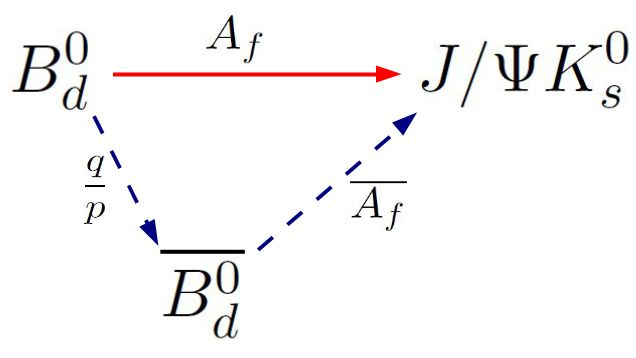
\includegraphics[width=0.5\textwidth]{interferenz}
\caption{Schema für die \CP-Verletzung in der Interferenz. Es interferieren die Amplituden für den direkten Zerfall (rot, durchgezogen) mit der Amplitude für den Zerfall nach vorheriger Mischung (blau, gestrichelt).}
\label{fig:interferenz}
\end{figure}
Der in dieser Arbeit betrachtete Zerfallskanal $B_d^0 \rightarrow J/\Psi K_s^0$ ist ein \CP-Eigenzustand. In Anlehnung an (\ref{eq:decay_amplitudes}) sind die Zerfallsamplituden hier - unter Vernachlässigung der \CP-Verletzung im Kaon-System - definiert als
\begin{align}
\nonumber A_f := \Braket{f|\text{\Bd}(t)\vphantom{\text{\Bdbar}}}, \qquad \overline{A_{f}} := \Braket{f|\text{\Bdbar}(t)}
\end{align}
Es wird außerdem die komplexe Größe
\begin{align}
\lambda_f := \frac{q\overline{A_f}}{pA_f} \label{eq:lambda}
\end{align}
definiert. Ausgehend von Gleichung (\ref{eg:b(t)}) sowie mit Hilfe der Gleichungen (\ref{eq:Gamma}), (\ref{eg:pq_approx}) und (\ref{eq:lambda}) gilt für die Zerfallsrate eines anfänglich reinen \Bd-Zustands:
\begin{align}
\nonumber &\Gamma (\text{\Bd} \rightarrow \JPsi\Kshort) \\
\nonumber &= \frac{1}{4}\left| (\e^{-\gamma_{\text{H}} t}+\e^{-\gamma_{\text{L}} t})A_f - \frac{q}{p}(\e^{-\gamma_{\text{H}} t}-\e^{-\gamma_{\text{L}} t})\overline{A_f}\right|^2 \\
&= \frac{1}{2} \left|A_f\right|^2\e^{-\Gamma t} \left[1+|\lambda_f|^2 + (1-|\lambda_f|^2)\cos(\Delta m_d t) - 2\mathrm{Im}(\lambda_f)\sin(\Delta m_d t)\right] \label{eq:bd}
\end{align}
Analog:
\begin{align}
\nonumber &\Gamma (\text{\Bdbar} \rightarrow \JPsi\Kshort) \\
&= \frac{1}{2} \left|A_f\right|^2\e^{-\Gamma t} \left[1+|\lambda_f|^2 -(1-|\lambda_f|^2)\cos(\Delta m_d t) + 2\mathrm{Im}(\lambda_f)\sin(\Delta m_d t)\right] \label{eq:bdbar}
\end{align}
Damit kann die vom Standardmodell prognostizierte \CP-verletzende Asymmetrie 
\begin{align}
\mathcal{A}_{\text{\CP}} :&= \frac{\Gamma (\text{\Bdbar} \rightarrow \JPsi\Kshort) - \Gamma (\text{\Bd} \rightarrow \JPsi\Kshort)}{\Gamma (\text{\Bdbar} \rightarrow \JPsi\Kshort) + \Gamma (\text{\Bd} \rightarrow \JPsi\Kshort)} \label{eq:cp_asymm_def}\\
&= -\frac{1-|\lambda_f|^2}{1+|\lambda_f|^2}\cos(\Delta m_d t) + \frac{2\mathrm{Im}(\lambda_f)}{1+|\lambda_f|^2}\sin(\Delta m_d t) \\
&= \CJPsi \cos(\Delta m_d t) + \SJPsi \sin(\Delta m_d t) \label{eq:cp_asymm}
\end{align}
berechnet werden. Da $\Ket{\JPsi\Kshort}$ ein fast reiner \CP-Eigenzustand ist, gilt $|\lambda_f| \approx 1$, womit sich jene hier zu
\begin{align}
\mathcal{A}_{\text{\CP}} \approx \mathrm{Im}(\lambda_f)\sin(\Delta m_d t)
\end{align}
vereinfacht. Folglich kann im B-Meson-System, insbesondere im Zerfall \linebreak\mbox{\Decaychannel} durch Messung der Asymmetrie-Amplitude $\SJPsi$ \CP-Verletzung in der Interferenz gemessen werden.
\begin{align}
\nonumber &\text{\CP-Verletzung in der Interferenz zwischen Mischung und Zerfall} \\ &\Longleftrightarrow \qquad \SJPsi = \mathrm{Im}(\lambda)\neq 0
\end{align}

\section{CKM-Formalismus}
Durch Austausch eines W$^{\pm}$-Bosons können Quarks ihren Flavour ändern. Dabei sind sie aber nicht an ihre jeweilige Generation gebunden, sondern können - wenn auch zum Teil stark unterdrückt - prinzipiell den Flavour einer jeden Generation annehmen. Ein kleines Beispiel: Der Eigenzustand $\Ket{u}$ der starken Wechselwirkung geht über den schwachen Prozess (Austausch eines W$^{\pm}$-Bosons) nicht in ein $\Ket{d}$ über, sondern vielmehr in eine Linearkombination aus $\Ket{d}$, $\Ket{s}$ und $\Ket{b}$, die im folgenden mit $\Ket{d'}$ bezeichnet wird. Allgemein werden die möglichen Linearkombinationen durch die Cabibbo-Kobayashi-Maskawa-Matrix (kurz: CKM-Matrix) beschrieben.
\begin{align}
\begin{pmatrix}
\Ket{d'} \\ \Ket{s'} \\ \Ket{b'}
\end{pmatrix}
=
\begin{pmatrix}
V_{ud} & V_{us} & V_{ub} \\
V_{cd} & V_{cs} & V_{cb} \\
V_{td} & V_{ts} & V_{tb} \\
\end{pmatrix}
\cdot
\begin{pmatrix}
\Ket{d} \\ \Ket{s} \\ \Ket{b}
\end{pmatrix}
\end{align}
Das Betragsquadrat eines jeden Matrixelementes $|V_{ij}|^2$ gibt dabei die Wahrscheinlichkeit für den Übergang eines Quarks $\Ket{i}$ in ein $\Ket{j}$ an. Da die $V_{ij}$ prinzipiell komplex sein können, gibt es zunächst 18 freie Parameter, die zu bestimmen sind. Diese Zahl reduziert sich zum einen um 5 relative Quarkphasen, die physikalisch nicht beobachtbar sind. Zum anderen reduziert die Forderung nach Unitarität der CKM-Matrix die Zahl der unabhängigen Parameter um 9, sodass am Ende 4 Parameter, 3 Euler Winkel sowie eine Phase, welche für die \CP-Verletzung verantwortlich ist, zu bestimmen sind. Die CKM-Matrix lässt sich näherungsweise durch die Wolfenstein-Parametrisierung darstellen:
\begin{align}
V_{\text{CKM}}=
\begin{pmatrix}
V_{ud} & V_{us} & V_{ub} \\
V_{cd} & V_{cs} & V_{cb} \\
V_{td} & V_{ts} & V_{tb} \\
\end{pmatrix}
=
\begin{pmatrix}
1-\frac{\lambda^2}{2} & \lambda & A\lambda^3(\rho-\im\eta) \\
-\lambda & 1-\frac{\lambda^2}{2} & A\lambda^2 \\
A\lambda^3(1-\rho-\im\eta) & -A\lambda^2 & 1
\end{pmatrix}
+ \mathcal{O}(\lambda^4)
\end{align}
Für den Zerfall von \Bd-Mesonen ist die Unitaritätsbedingung
\begin{align}
V_{ud}V_{ub}^* + V_{cd}V_{cb}^* + V_{td}V_{tb}^* = 0
\end{align}
von besonderer Bedeutung. Man kann die einzelnen Summanden nun in der $(\rho,\eta)$-Ebene auftragen und erhält dabei ein sogenanntes Unitaritätsdreieck. Es wird so normiert, dass die Unterseite bei (0,0) beginnt und bei (1,0) endet (siehe Abb. \ref{fig:unitarity}). Die obere Ecke liegt dann bei $(\overline{\rho}, \overline{\eta})$, wobei $\overline{\rho} = \rho(1-\lambda^2/2)$ und $\overline{\eta} = \eta(1-\lambda^2/2)$ gemäß der Wolfenstein-Parametrisierung sind. Die Winkel des Dreiecks erhält man über
\begin{align}
\alpha = \text{arg}\left[-\frac{V_{td}V_{tb}^*}{V_{ud}V_{ub}^*}\right], \qquad
\beta = \text{arg}\left[-\frac{V_{cd}V_{cb}^*}{V_{td}V_{tb}^*}\right], \qquad
\gamma = \text{arg}\left[-\frac{V_{ud}V_{ub}^*}{V_{cd}V_{cb}^*}\right].
\end{align}
\begin{figure}[hptb]
\centering
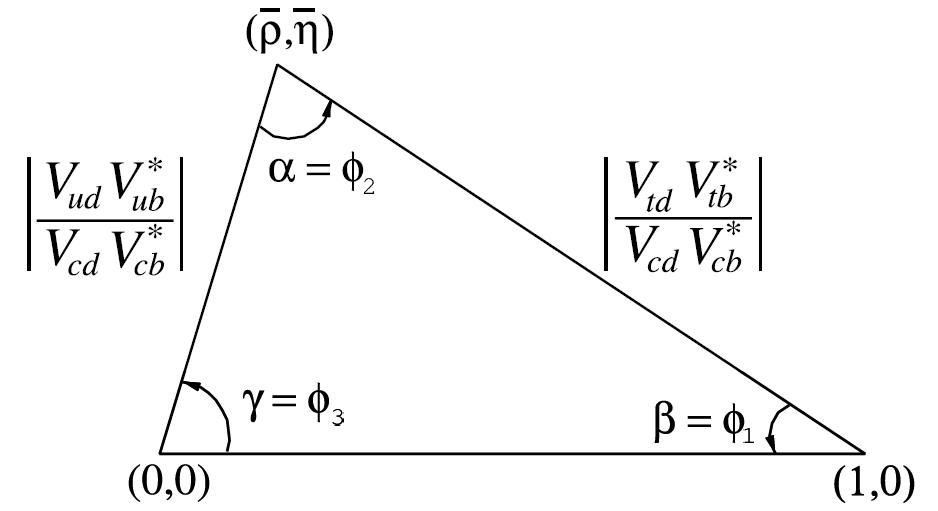
\includegraphics[width=0.5\textwidth]{dreieck}
\caption{Unitaritätsdreieck, entnommen von \cite{dreieck}}
\label{fig:unitarity}
\end{figure}
Das Standardmodell stellt für den hier untersuchten Zerfallskanal eine Beziehung zwischen dem Winkel $\beta$ und der komplexen Größe $\lambda_f$ aus Gleichung (\ref{eq:lambda}) her \cite{nir,noguchi}:
\begin{align}
&\lambda_f = \underbrace{\frac{V_{td}V_{tb}^*}{V_{td}^*V_{tb}}}_{\frac{q}{p}} \underbrace{\frac{V_{cd}^*V_{cb}}{V_{cd}V_{cb}^*}}_{\frac{\overline{A_f}}{A_f}} = \e^{2\im\beta} \\
\Longrightarrow \quad &\SJPsi = \mathrm{Im}(\lambda_f) = \sin(2\beta).
\end{align}
Durch Messung der Amplitude der \CP-Asymmetrie kann man direkte Rückschlüsse auf den CKM-Winkel $\beta$ ziehen, der wesentlicher Bestandteil des Standardmodells ist \cite{nir}.